\documentclass[a4paper]{article}
\usepackage[english]{babel}
\usepackage[utf8x]{inputenc}
% package for including graphics with figure-environment
\usepackage{graphicx}
\usepackage{parskip}
\usepackage{amssymb}
\usepackage{mathbbol}
\usepackage{amsmath}
\DeclareMathOperator*{\minimize}{minimize}
%\usepackage{verbatim}
\usepackage{hyperref}
\usepackage[natbibapa]{apacite}
\usepackage{geometry}
\geometry{
 a4paper,
 %total={170mm,257mm},
 left=30mm,
 top=30mm,
 right = 20mm,
 bottom = 30mm
 }
% colors for hyperlinks
% colored borders (false) colored text (true)
\hypersetup{colorlinks=true,citecolor=black,filecolor=black,linkcolor=black,urlcolor=black}

% package for bibliography
\PassOptionsToPackage{authoryear,round}{natbib}
% package for header
\usepackage[automark]{scrpage2}
\usepackage{braket}
\usepackage{enumerate}
\pagestyle{scrheadings}
\ihead[]{Mark Fingerhuth}
\ohead[]{\today}
\cfoot[]{\pagemark} 
\setheadsepline[160mm]{0.3mm}

% Defining some new mathematics commands
\newcommand*{\colvec}[1]{\begin{pmatrix}#1\end{pmatrix}}
\newcommand*{\0}{$\ket{0}$}
\newcommand*{\1}{$\ket{1}$}


\begin{document}
\title{
\vspace{1cm}
\begin{figure}[!ht]
\centering

\includegraphics[width=0.5\textwidth]{MSC2.png}
\end{figure}
\vspace{0.3cm}
\begin{figure}[!ht]
\centering

\includegraphics[width=0.5\textwidth]{logo.jpeg}
\end{figure}
\vspace{2cm}
\Huge{\bf{Research Proposal for the} \\ Experimental Implementation of Quantum Machine Learning Algorithms \\}}
\vspace{3cm}
% Insert here your name and correct mail address
\author{\Large \href{mailto:m.fingerhuth@student.maastrichtuniversity.nl}{Mark Fingerhuth}
}
\date{
\today \\
\vspace{2.0cm}
In partial fulfillment of the requirements for the degree Bachelor of Science (BSc) at Maastricht University. \\
\vspace{1cm}
In collaboration with the Quantum Research Group at the University of KwaZulu-Natal Durban. Under supervision of Prof. Petruccione, Quantum Research Group at UKZN, and internal supervisor, Dr. Fabrice Birembaut, Maastricht Science Programme, Maastricht University.
}
% In partial fulfillment of the requirements for the degree Bachelor of Science, Maastricht University. 
\maketitle
\setlength{\parindent}{0pt}

%Braket package: $\braket{0|0}$

\vspace{10.0cm}
\begin{abstract}

% >> this should be a nice concise summary of the entire proposal
Mixtape tote bag quinoa, deep v ramps organic pabst. Cliche trust fund twee lo-fi, lumbersexual sustainable skateboard brunch keytar edison bulb. Try-hard blue bottle meggings fashion axe, gentrify freegan PBRB. Squid retro viral, shoreditch sriracha salvia kogi chia. Celiac tumblr thundercats, williamsburg literally etsy man braid franzen flannel chambray raw denim. Try-hard woke retro intelligentsia. Af actually synth coloring book hoodie tumeric, knausgaard paleo butcher.

\end{abstract}
	\newpage
	\tableofcontents
	\newpage

\section{Introduction}
\label{sec:introduction}

%>> Introduce the TOPIC (QML) not the (HYPO)THESIS!

The ability to understand spoken language, to recognize faces and to distinguish different types of fruit comes naturally to humans, even though these processes of pattern recognition and classification are inherently complex. Machine learning (ML), a subtopic of artificial intelligence, is concerned with the development of algorithms that mimic these mechanisms, thereby enabling computers to find and recognise patterns in data and classify unknown inputs based on previous training with labelled inputs. Such algorithms paved the way for e.g. human speech recognition, recommendation engines as used by Amazon and prediction algorithms that can predict heart disease from real-time electrocardiograms \citep{acharya2015integrated}.

According to \cite*{bigdata}, every day approximately 2.5 quintillion (${10}^{18}$) bytes of digital data are created. This growing number implies that every area dealing with data will eventually require advanced algorithms that can make sense of data content, retrieve patterns and reveal correlations. However, most ML algorithms involve the execution of computationally expensive operations and doing so on large data sets inevitably takes a lot of time \citep{bekkerman2011scaling}. Hence, it becomes increasingly important to find efficient ways of dealing with big data and/or reduce the computational complexity of the algorithms.

A promising solution is the use of quantum computation which has been researched intensively in the last decades. Quantum computers (QCs) use quantum mechanical systems and their special properties to manipulate and process information in ways that are impossible to implement on classical computers. The quantum equivalent to a classical bit is called a quantum bit (or qubit) and additionally to being in either state they can be in a linear superposition of \0 and \1. This peculiar property gives rise to so called quantum parallelism, which enables the execution of certain operations on many quantum states at the same time. However, despite this obvious advantage the real difficulty in quantum computation lies in the retrieval of the computed solution since a measurement of a qubit collapses it into a single classical bit and thereby destroys information about its previous superposition. Several quantum algorithms have been proposed that provide exponential speed-ups when compared to their classical counterparts with Shor's prime factorization algorithm being the most famous \citep{shor1994}. Hence, quantum computation bears the potential to vastly improve computational power, speed up the processing of big data and solve certain problems that are practically unsolvable on classical computers. 

%for the QML toolbox to be complete a quantum algorithm to solve systems of linear equations is needed since most ML algorithms rely on solving those.

Considering these advantages, the combination of quantum computation and classical ML into the new field of quantum machine learning (QML) seems almost natural. However, since most ML algorithms rely on solving some system of linear equations a corresponding quantum algorithm is required for QML to become achievable. \cite{HHL2009} were first to describe such an algorithm (referred to as HHL-algorithm) which since has become a subroutine in many QML algorithms. There are currently two main ideas on how to merge quantum computation with ML, namely a) running the classical algorithm on a classical computer and 'outsourcing' only the computationally intensive task to a QC or b) executing the quantum version of the entire algorithm on a QC. Current QML research mostly focusses on the latter by developing quantum algorithms that tab into the full potential of quantum parallelism.

%QML
%- the unification or symbiosis of ML and QC comes naturally when considering the vast speed-ups that could be gained through implementing ML on QCs
%- this relatively new research field is called QML and is largely based on the discovery of the HLL algorithm
%- two possibilities: 1. run entire algorithm on QC or 2. run computationally exhaustive subroutines on QC and the rest on a CC


%ML

%- machine learning as a subarea of artificial intelligence is all about teaching/training a computer on how to recognise patterns, classify unknown information and ultimately learn from given input data
%- important for prediction algorithms, recommendation engines, expert machines (e.g. Watson) and computer vision or speech recognition
%- cite the amount of data humans create per year >> this huge amount of data requires advanced analysis in order to make sense of it
%- machine learning algorithms are usually very computationally exhaustive and when increasing the amount of data the computation time increases (exponentially???) >> maybe give the example of how long it took AlphaGo to be trained

%Quantum

%- quantum computation has become a very promising research area
%- it exploits/uses quantum mechanical systems to manipulate information and since quantum mechanics allows for superpositions it makes quantum parallelism possible / things like interference can be used to our benefit
%- offers the possibility of vastly boosting our computational power and enrich the space of solvable problems e.g. optimization problems (might be able to solve some P and NP problems) >> check this exactly
%- quantum mechanics essentially is 'applied linear algebra in complex vector spaces' and since classical computation is all about manipulating vectors and matrices the usefulness of QM for computation becomes obvious

\newpage

\subsection{Motivation}
\label{subsec:motivation}

Classical ML is a very practical topic since it can be directly tested, verified and implemented on any commercial classical computer. So far, QML has been of almost entirely theoretical nature since the required computational resources are not in place yet. QML algorithms often require a relatively large number of error-corrected qubits and some sort of quantum data storage such as the proposed quantum random access memory (qRAM) \citep{qRAM}. However, to date the maximum number of superconducting qubits reportedly used for calculation is nine, the D-Wave II quantum annealing device delivers 1152 qubits but can only solve a narrow class of problems and a qRAM has not been developed yet \citep{hydrogensimulation, dwave2}. Furthermore, qubit error-correction is still a very active research field and most of the described preliminary QCs deal with non error-corrected qubits with short lifetimes and are, thus, impractical for large QML implementations.

Until now there has been only three experimental verifications of QML algorithms that provide proof-of-principle. \cite{Li2015} successfully distinguished a handwritten six from a nine using a quantum support vector machine on a four-qubit nuclear magnetic resonance test bench. In addition, \cite{Cai2015} were first to experimentally demonstrate quantum machine learning on a photonic QC and showed that the distance between and the inner product of two vectors can indeed be computed quantum mechanically. Lastly, \cite{Riste2015} solved a learning parity problem with five superconducting qubits and found that a quantum advantage can already be observed in non error-corrected systems.

%Consequently,
Considering the large gap between the number of proposed QML algorithms and experimental realisations of scaled-down QML problems, it remains important to find QML problems which can already be implemented on currently available quantum technology. Thus, the purpose of this study is to provide proof-of-principle implementation of selected QML algorithms on small datasets. This is a step in the attempt to shift QML from a purely theoretical research area to a more applied field such as classical ML. Furthermore, this can also lead to verification or falsification of the claims and assumptions made in the field of QML. 

%Does this belong here?
%The proposed research will identify small ML problems and find suitable datasets, that can already be solved using QML algorithms and current quantum computing technology. Earlier this year, technology company IBM has provided the public with access to their experimental quantum processor containing five non error-corrected superconducting qubits. Investigated will be two algorithms proposed by \cite{Schuld2014, Schuld2016} that focus on supervised pattern classification based on linear regression and vector distance measurements.

%>> what is your point? what exactly do you wanna do and why? why does it makes sense?
%>> (Background and literature review/current state)

%- ML is a very hands-on, practical and applied topic whereas QML has been almost entirely theoretical so far since the computational resources are not in place yet
%- mostly of theoretical nature since QML algorithms often require large amounts of qubits, error-corrected qubits and some sort of qRAM
%- there have been only a handful of attempts to experimentally implement QML algorithms as proof-of-concept studies ( cite Li and other fellows)
%- it is therefore important to continue along this line and to find small ML subproblems which can already be implemented on currently available technology in an attempt to unify the practical research area of ML with the theoretical side of QML and verify the claims and assumptions of the QML researchers 
%- there are many proposed quantum Machine Learning algorithms which should hypothetically work but who have not been implemented or verified experimentally yet
%- Finding very small machine learning problems which can be implemented on IBM’s QC would constitute a proof-of-concept for the quantum machine learning age. This is crucial for further research to be funded and supported since it shows that an upscaling of QCs will eventually lead to huge speed ups in ML routines and therefore 			revolutionize the handling of big data

\subsection{Research Question}
\label{subsec:researchquestion}

In light of the theoretical nature of current QML research and the small number of experimental realizations, this research will address the following question:
 
\centering\textbf{How can theoretically proposed quantum machine learning algorithms be implemented on state-of-the-art quantum technology?}

%Alternatives:
%Is it possible to experimentally demonstrate that two QML algorithms proposed by \cite{Schuld2014, Schuld2016} can already solve a small ML problem using classical simulation or IBMs quantum processor?
%Is it possible to already implement and solve a small ML problem on IBMs publicly available quantum computer?

\flushleft
The following sections will outline the steps required and the tools used in order to answer this research question. 

\newpage
\subsection{Research Objectives}
\label{subsec:researchobjectives}

The main objective of this research is to demonstrate that QML algorithms can already be used for solving small problems on currently available quantum technology. Even though this might seem trivial at first, there are many problems that are often not addressed in the proposals of QML algorithms such as the encoding of data, the influence of quantum noise and the restrictions on the data type (e.g. uniformly distributed or sparse data sets only). All theses issues have to be addressed when implementing QML algorithms experimentally and thus consitute the major challenges during this study. 
%not sure about the usefulness of the last sentence
Ideally, the outcome will already demonstrate observable quantum advantages over the classical algorithms, provide supporting evidence for the claim that QML can indeed be used to solve ML problems and that the increasing number of qubits will bring the expected speed-ups in computation.

%Proof-of-principle
%Demonstrating that some QML algorithms can already be used for solving small problems

%tackling the many problems that are often not adressed in QML algorithm papers like data encoding, quantum noise, the constitution of the data (sparse, low-rank, uniformly distributed) by implementing it from start to end and having to encount them

%implement the circuit in a quantum system (ideally on a real QC otherwise simulate it in Liquid)
%many QML algorithms assume the data to already be prepared in some particular quantum data format and also assume all kind of other things
%This includes a) the preprocessing of data, b) the preparation of a suitable quantum state containing the training data and the to be classified data, 
%c) the execution of a quantum circuit and finally d) the retrieval of the solution to the problem.
%shall I give examples for such small ML problems?
%Thereafter, 
%identify small ML problems and find suitable datasets, that can already be solved using QML algorithms and current quantum computing technology. Earlier this year, technology company IBM has provided the public with access to their experimental quantum processor containing five non error-corrected superconducting qubits. Investigated will be two algorithms proposed by \cite{Schuld2014, Schuld2016} that focus on supervised pattern classification based on linear regression and vector distance measurements.
%Essentially: find a QAlg + a downscaled ML problem + a dataset
%classification problems such as classifying handwritten digits/colours or fitting functions onto small datasets could be scaled down and executed on 5 Qbits

\newpage
		
\section{Research Methods}
\label{sec:researchmethods}

%>> how are you going to approach the problem? what tools do you wanna use?

%%WHAT ALGORITHMS AND WHAT DO THEY DO???

% Making clear that only 2 algorithms are used!
The proposed research will be solely based on the two QML algorithms described in \cite{Schuld2014, Schuld2016}. Firstly, \cite{Schuld2014} is a quantum version of the distance weighted $k$-nearest neighbour (KNN) algorithm. For clarification, let us consider a training data set ${D}_{T}$ consisting of five vectors ${v}_{0}, {v}_{1},...$ that are each either assigned to class $A$ or $B$. Classical KNN is a non-parametric classifier that given an unclassified input vector $x$ considers the $k$ nearest neighbours (using a predefined measure of distance) and classifies $x$, based on a majority vote, as either $A$ or $B$. Thereby, $k$ is a positive integer and is usually chosen to be small. In the case of $k = all$, input vector $x$ would simply be assigned to the class with the most members. In this case, the training vectors can be given distance-dependent weights (such as $1/distance$) in order to increase the influence of closer vectors over more distant ones. The advantage of the quantum version is the parallel computation of the distance between each training vector and the input vector as well as contracting distance computation and the weighing into one computational step.

Next, \cite{Schuld2016} details a quantum algorithm based on least-squares linear regression. In contrast to the discrete classes ($A$ or $B$) used in kNN, this algorithm focusses on continuous outputs and the task is to learn how to map inputs to continuous outputs after being trained on a training data set.
%needs writing!
%explain linear regression and sketch the quantum algorithm

%%CHOOSING SMALL PROBLEMS AND GENERATING THE DATASET
The first step towards their experimental implementation will be the identification of one or several small ML problems that can be executed on maximally nine qubits. For example, this might include the characterization of colours or differentiation of digits or letters. It thereby plays an important role if the respective ML problem can be approached using a very small dataset such as the average pixel brightness or the ratio of pixels above and below the bisector of the image. Ideally, the data should be representable as a 2-D vector such that it requires only a few qubits to encode the information quantum mechanically.

%%THE TOOLS
%maybe describe the possible tools here (liquid, IBM, python, etc.)
%shortly introduce the IBM QC and what Liquid is
There are two types of tools available for the implementation of the QML algorithms. Firstly, since current state-of-the-art quantum technology uses maximally nine qubits, a classical computer can still be used to simulate the behaviour of the QC. Such a software architecture is provided by Microsoft Research which has released the quantum simulation toolsuite Liqui$\ket{}$ based on the programming language F\#. There are many more QC simulator toolsuites available and the decision which one to use depends on the selected QML problem and dataset \citep{quantiki}.

Secondly, earlier this year technology company IBM has enabled public access to their experimental quantum processor containing five non error-corrected superconducting qubits. Instead of only simulating on classical hardware, this opens up the possibility of executing the QML algorithm on actual quantum hardware. If it is possible to make use of IBM's QC is highly dependent on the dataset chosen. Furthermore, until this point it remains unclear if the algorithm in \cite{Schuld2016} can be executed using five qubits only.

%%THE PROBLEM OF ENCODING THE DATA INTO QUANTUM STATES >> REFERENCE SOME PAPERS HERE
Both algorithms assume that the classical data is readily available in the form of quantum states. Hence, the first crucial step will be translating the classical data into such states, constituting the first challenge since it is a non-trivial and still researched topic. The quantum version of the distance weighted kNN requires a binary data string of length $n$ to be encoded one to one into $n$ qubits. This will be referred to as \textit{qubit encoding}. A possible algorithm for this type of data encoding was proposed by \cite{ventura1999initializing}. The quantum linear regression algorithm is based on so called \textit{amplitude encoding}, where the classical data is written into the amplitudes of quantum states which is more difficult to achieve than qubit encoding. Amplitude encoding is still a very active field of research and until now it can only be done with relatively uniform data sets. \cite{grover2002creating} described such an algorithm and special attention will be paid in choosing a suitable uniform dataset when using this algorithm.

%%DESIGNING THE QUANTUM CIRCUITS
Next, two separate quantum circuits consisting of quantum logic gates will be designed that accurately represent the two QML algorithms as outlined in the paper of \cite{Schuld2014, Schuld2016}. Each quantum circuit is then combined with its respective data encoding circuit. Finally, the computed solution needs to be retrieved by measuring specific qubits. By repeating the execution of the algorithms, a probability distribution over the qubit measurements is obtained that represents the solution to the given problem.

To summarize, the steps needed for the successful implementation of a QML algorithm are given below.

\begin{enumerate}
\item Find a small implementable ML problem
\item Generate or find a suitable dataset
\item Encode the classical data into quantum states
\item Design a quantum circuit representing the QML algorithm
\item Execute the entire quantum circuit multiple times
\item Retrieve the solution from the resulting probability distribution
\end{enumerate}

\section{Timeline}
\label{sec:timeline}

The projected timeline for the proposed bachelor thesis research is given below.

\begin{figure}[!ht]
\centering
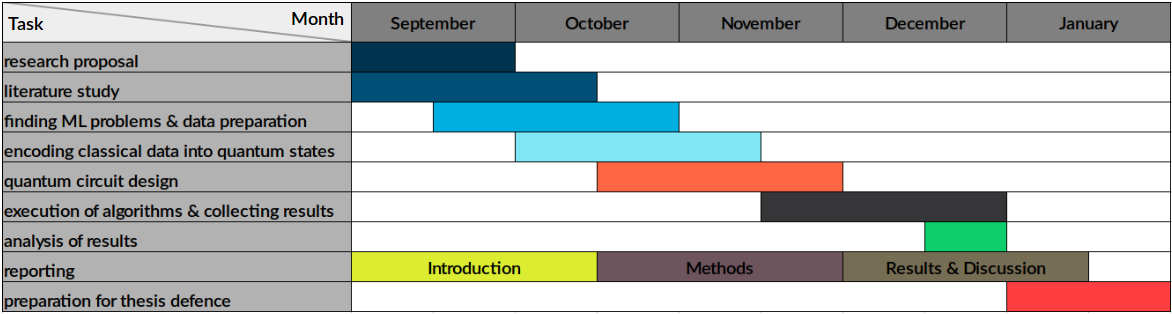
\includegraphics[scale=0.385]{ready_timeline.png}
\caption{Projected timeline for proposed research}
\end{figure}

\section{Research Impact}
\label{sec:research impact}
%is this really needed?
Successful proof-of-principle studies are crucial for further research to be funded and supported since it shows that an upscaling of quantum computational power will eventually lead to at best exponential speed ups compared to classical ML and hence has the potential to revolutionize the handling of big data.

\section{Conclusion}
\label{sec:conclusion}
axidermy edison bulb plaid, chia swag organic roof party shabby chic raw denim tilde waistcoat. Swag everyday carry iPhone, pitchfork pop-up ethical blog small batch la croix before they sold out chartreuse chia gastropub craft beer crucifix. Occupy mustache organic tumblr, scenester cred listicle kombucha lumbersexual. Crucifix tumeric bushwick, organic unicorn ugh food truck 90's echo park freegan mumblecore chia shabby chic. Keytar actually intelligentsia mumblecore, ugh selvage schlitz tousled iPhone cray paleo wayfarers snackwave viral humblebrag. Subway tile pop-up squid church-key craft beer. Church-key la croix cornhole kitsch 8-bit gluten-free.

\newpage
\section{References}
\begingroup
\renewcommand{\section}[2]{}%
\bibliographystyle{apacite}
\bibliography{proposal}
\endgroup

%\newpage

%\section{Appendix}


\end{document}